\documentclass[journal]{IEEEtran}
\usepackage{iftex}
\ifPDFTeX
\usepackage[T1]{fontenc}\usepackage[utf8]{inputenc}
\else
\usepackage{fontspec}\setmainfont{Times New Roman}\setsansfont{Arial}\setmonofont{Courier New}
\fi
\usepackage{cite,amsmath,amssymb,amsthm,graphicx,booktabs,array,tabularx,xspace,url}
\usepackage[hidelinks]{hyperref}
\newcommand{\MSLE}{\textsc{M-SLE}\xspace}
\newcommand{\HD}{\operatorname{HD}}
\newcommand{\Adv}{\operatorname{Adv}}
\newtheorem{proposition}{Proposition}
\newtheorem{theorem}{Theorem}
\begin{document}
\title{Masked Synchronized Locator Evolution for Re-Keyable Private Face Identification}
\author{Beibut Amirgaliyev,~\IEEEmembership{Member,~IEEE}, and Serzhan Ossenov,~\IEEEmembership{Member,~IEEE}%
\thanks{The authors are with the Research and Innovation Center Smart City, Astana IT University, Astana 010000, Kazakhstan (e-mail: beibut.amirgaliyev@astanait.edu.kz; 255351@astanait.edu.kz).}%
\thanks{Serzhan Ossenov is the corresponding author.}}
\markboth{IEEE Transactions on Biometrics, Behavior, and Identity Science, 2026}{Amirgaliyev and Ossenov: Masked Synchronized Locator Evolution}
\maketitle
\begin{abstract}
Renewing a protected biometric template also requires maintaining its association with the search index. Masked Synchronized Locator Evolution (\MSLE) couples identity-conditioned binary-template masking with a verified update of independently shared database and index locators. Matching preserves Hamming scores over the same candidate set; direct mask-to-mask rotation requires neither a face sample nor a persisted raw root. The revised protocol verifies both template renewal and the resulting database-index relation before selecting the next complete state. Confidentiality requires secret mask keys. We give an explicit private retrieval procedure, a completeness certificate with exhaustive fallback, and a fixed-scan implementation that hides memory addresses. Matched float/binary experiments quantify frontend loss rather than attributing all utility preservation to the complete recognition pipeline. Twenty LFW splits extend the gallery to 4096 identities; binary Rank-1 falls from 0.9849 at 128 to 0.9367 at 4096, compared with 0.9531 for float embeddings at 4096. Independent calibration and unenrolled identities assess rejection. Complete five-party measurements include masking, verification, row shuffling and share refresh, and compare against shared roots and oblivious sort/merge. The contribution is a reproducible lifecycle contract and relational-leakage analysis, with explicit computational and deployment costs.
\end{abstract}
\begin{IEEEkeywords}
Biometric template protection, private face identification, key rotation, secure multi-party computation, private index, unlinkability.
\end{IEEEkeywords}

\section{Introduction}
An encrypted or secret-shared face database must remain usable when its protection keys change. Updating only the template can leave a stale private index; updating only the index can retain a stable protected biometric object. We study the joint transition of a binary template, redundant semantic locator copies and their hidden relation. The intended operation is a key-epoch change without requesting another face sample.

Our motivating leakage example concerns a gallery exposed as protected values. XORing every root with one epoch-wide mask changes individual values but preserves every pairwise Hamming distance. A row can therefore be described by its sorted distances to the other rows. Matching these signatures across shuffled epochs can recover correspondence even when direct old/new similarity is uninformative. Identity-conditioned masks remove this common isometry. This observation is about exposed protected values; ordinary Shamir sharing already hides raw roots against a below-threshold adversary.

\MSLE stores $\mathbf c_i^e=\mathbf b_i\oplus G(K_e,\ell_i^e)$ and masks each probe separately for each compared identity. It updates templates and independently held locator copies inside MPC, checks the proposed state, and jointly selects the accepted epoch. Its novelty is the explicit cross-layer invariant and its implementation and evaluation, rather than a new PRF, a stronger MPC corruption threshold, or the existence of root-free ciphertext updates.

The paper makes four contributions precise: (i) an inherited/new-state comparison and a template-binding check in addition to locator/index consistency; (ii) a secret-key confidentiality argument with an explicit concrete circuit; (iii) private candidate retrieval with measured recall, capacity and certified fallback; and (iv) complete secure-system and paired biometric evaluation. The fixed-scan backend is a privacy reference implementation. It does not provide sublinear query time.

\section{Related Work and Simpler Alternatives}
FaceNet and VGGFace2 provide the evaluated embedding frontend~\cite{schroff2015facenet,cao2018vggface2}. Cancelable and protected representations include PolyProtect, learned non-linkable representations and stable hashes for preselection~\cite{hahn2022polyprotect,pinto2021securetriplet,osorioroig2022stablehash}; broader surveys emphasize separate utility, irreversibility and unlinkability criteria~\cite{krivokuca2023survey}. Their transformation and reissuance mechanisms differ. We do not infer an absence of re-keying merely because a method does not implement our joint index transaction.

Private identification systems protect matching through cryptographic computation~\cite{franz2009privacyface,osadchy2010scifi}. HERS compresses learned representations and searches encrypted galleries using homomorphic encryption~\cite{engelsma2022hers}. It is an important scalable encrypted-search reference, with a different numeric representation, key architecture and workload. Its reported large-gallery throughput is not a comparable baseline for a five-party verified epoch transition. We compare functionalities and assumptions, not unrelated runtime numbers.

Updatable encryption explicitly supports ciphertext renewal without decrypting data at the updating server; Lehmann and Tackmann formalize post-compromise and forward security with update tokens~\cite{lehmann2018updatable}. Thus protected-to-protected renewal itself is established functionality. Our secret-key, clean-snapshot statement is not their post-compromise guarantee. Conventional randomized encryption can also store renewable templates; MPC can decrypt, compare and re-encrypt transiently while synchronizing the same index. We make no impossibility or superiority claim against this design.

MPC, Shamir sharing, proactive refresh, shuffles, ORAM and private joins supply the required components~\cite{shamir1979share,keller2020mpspdz,herzberg1995proactive,stefanov2013pathoram,mohassel2020joins}. Earlier SLE is an \emph{internal, unpublished predecessor}, not a prior peer-reviewed result. Its frozen source is included in the reproducibility artifact. It stored shared binary roots and already used synchronized locator evolution, relation fingerprints and joint state selection. Table~\ref{tab:extension} separates inherited components from additions.
\begin{table}[t]
\caption{Internal SLE predecessor and the evaluated extension.}
\label{tab:extension}\centering\small
\begin{tabularx}{\columnwidth}{p{.25\columnwidth}XX}
\toprule Component & Internal SLE & \MSLE \\
\midrule Persistent root & $[\mathbf b_i]$ & $[\mathbf c_i^e]$ \\
Epoch secrets & locator key & locator key and independent mask keys \\
Locator evolution & inherited & same permutation on independent copies \\
Relation invariant & root-index tuples & proposed decoded template-index tuples \\
Renewal binding & stable root & verify old/new template equation \\
Commit/refresh & inherited & includes template and mask-key bundle \\
Query & root Hamming & candidate-conditioned Hamming \\
\bottomrule
\end{tabularx}
\end{table}

The strongest simple comparison is shared raw roots with proactive refresh under the same five-party threshold. It already hides roots, metadata and transcripts and can support the same index transaction. \MSLE removes raw roots from persistent logical state and additionally protects \emph{exposed masked values while mask keys remain secret}. The mask layer is standard locator-conditioned PRF encryption at the value level. Its benefit matters only when such exposure is in scope; it does not strengthen below-threshold MPC privacy. We measure its extra cost against this baseline.

\section{State, Adversary and Concrete Construction}
Five parties use degree-two Shamir sharing over $\mathbb F_p$; any three shares reconstruct. The evaluated MP-SPDZ backend is passive~\cite{keller2020mpspdz}. The proof assumes at most two corrupt parties, private authenticated channels, and correct protocol execution. Fault injection tests application-level consistency, not malicious MPC security.

For a normalized embedding $\mathbf z$, the binary root is $b_j=\mathbf1[z_j\ge0]$. A gallery root is the sign of the mean of two embeddings. A row contains shared locator $\ell_i$, masked root $\mathbf c_i$, identity label and a unique stable tie tag. Tie tags remain attached to identities during shuffling. The index holds a validity bit and independent locator copy in each padded slot. A root has $B=d/w$ blocks; bucket $(g,v)$ contains the locators whose block $g$ equals $v$. All dimensions and public capacities are disclosed. Enrollment rejects insufficient capacity and requires distinct locators; it never silently truncates buckets.

The clean-snapshot adversary may see unordered masked-value sets. It does not receive mask keys, locators, label mappings, stable row identifiers or index bucket contents. Query outputs and accept/reject bits can themselves reveal identity information; unlinkability is claimed only for snapshot assignments consistent with the \emph{same allowed leakage}, not for arbitrary identity-revealing interactions. A complete key/locator/template compromise recovers the root. A secret locator with an exposed mask key is \emph{not} covered by our PRF argument.

Secure initial sharing is assumed. In the executable storage experiment, an external trusted fixture prepares a valid protected state and gives each computing party one degree-two Shamir evaluation per field. The parties privately input these evaluations, interpolate inside MPC and store fresh state shares. The fixture knows the initial public-test roots and keys and is outside the party-corruption model. Subsequent transitions and queries load each party's own share file; plaintext database, index and old keys are not resupplied to a computing party.

\begin{table}[t]
\caption{Corrected executable parameters. Full constants and vectors are released.}
\label{tab:parameters}\centering\small
\begin{tabularx}{\columnwidth}{p{.33\columnwidth}X}
\toprule Item & Value \\
\midrule Field & $p=2^{128}-3637247$, prime \\
Permutation & cubic MiMC, 81 rounds; $\gcd(3,p-1)=1$ \\
Round constants & $c_0=0$; SHAKE rejection-sampled constants \\
Epoch keys & nine independent uniform elements of $\mathbb F_p$ \\
Key generation & sum of five independent full-field contributions per key \\
512-bit mask & eight independent keyed permutations, low 64 bits of each output \\
Bit extraction & canonical 128-bit known-prime decomposition \\
Relation challenges & two independent $(r,\alpha,\beta)\in\mathbb F_p^3$ \\
MPC parameters & five parties, threshold two; statistical parameter 80 \\
\bottomrule
\end{tabularx}
\end{table}

MiMC follows the cubic construction of Albrecht et al.~\cite{albrecht2016mimc}. In each round $x\leftarrow(x+k+c_j)^3$; the output adds $k$. The invertible cubing map makes the full circuit a permutation. The round count is at least $\lceil\log_3 p\rceil$. For locator evolution use key $k_0$; for mask word $h$ use independent key $k_h$, $1\le h\le8$, at the locator input. Independence avoids an unstated related-key or additive-domain-separation assumption. We assume this concrete keyed permutation is secure; the round formula and 128-bit field alone are not a security proof. The separate SHAKE-256 lifecycle simulation uses its released domain string and key/locator serialization and requires a corresponding secret-key pseudorandomness assumption. Its timings are never used as MPC performance.

\section{Protocol and Exactness}
\subsection{Matching and Candidate Retrieval}
For a probe $\mathbf q$ and candidate $i$, compute
\begin{equation}
\mathbf q_i^e=\mathbf q\oplus G(K_e,\ell_i^e),\qquad
d_i=\HD(\mathbf c_i^e,\mathbf q_i^e).
\end{equation}
\begin{proposition}[Same-candidate exactness]
For every fixed candidate set, protected and binary-root scores coincide. Rankings and threshold decisions coincide when the same stable tie tags are used.
\end{proposition}
\begin{proof}
For every bit, $(b\oplus m)\oplus(q\oplus m)=b\oplus q$. Summation preserves Hamming distance. Deterministic selection uses identical scores and tie tags.
\end{proof}
This proposition does not establish retrieval recall or equality with float recognition.

For each query block, select its bucket, union all valid locators and remove duplicates. The actual private reference circuit computes secret one-hot bucket flags, scans \emph{every padded slot}, compares full-field locators with every gallery locator and ORs matches. Retrieval costs $O(NM)$ full-field comparisons for $M$ slots. Candidate identities and candidate count stay secret. It scores the full gallery on the same public schedule and selects between candidate and exhaustive winners with a secret multiplexer. Consequently, a data-dependent fallback does not expose a change of memory trace or work. This construction is expensive but concrete; a faster ORAM-based implementation is not claimed.

\begin{proposition}[Certified exhaustive agreement]
If the index relation is complete and capacity is sufficient, an omitted record has Hamming distance at least $B$. The candidate winner is therefore also the exhaustive winner if its distance is strictly less than $B$, or if all records were retrieved. Otherwise use exhaustive fallback.
\end{proposition}
\begin{proof}
An omitted root differs from the probe in at least one bit in every block. Its distance is at least $B$. A candidate distance strictly below $B$ excludes both a better omitted record and an omitted tie. Exhaustive fallback handles the other cases.
\end{proof}
The strict inequality is needed for ties. The CPU retrieval study additionally records queried-overflow fallback for deliberately undersized indices; the secure backend instead rejects such enrollment. Main closed-set biometric comparisons use exhaustive search. Candidate recall and agreement are separate measurements.

\subsection{Verified Epoch Transition}
Let independent fresh epoch keys define
\begin{align}
\ell_i'&=\Pi_{k_0'}(\ell_i),\\
\mathbf c_i'&=\mathbf c_i\oplus G(K_e,\ell_i)\oplus G(K_{e+1},\ell_i').\label{eq:renew}
\end{align}
Every index locator copy is passed independently through the same permutation. No row-to-row pointer map is needed. The root is not a transition input. It can occur on transient secret wires while deriving bucket membership.

Before commit, verify \emph{both} (a) Eq.~\eqref{eq:renew} for every proposed template bit, and (b) the complete index multiset derived from $\mathbf c_i'\oplus G(K_{e+1},\ell_i')$. This prevents an index-consistent but incorrectly re-keyed template from being accepted. For $x=(\ell,g,v)$ define $E_{\alpha,\beta}(x)=\ell+\alpha g+\beta v$. For each of two independent challenges compare
\begin{equation}
\prod_{x\in\mathcal R_{\rm expected}}(r-E_{\alpha,\beta}(x))
=\prod_{x\in\mathcal R_{\rm proposed}}(r-E_{\alpha,\beta}(x)).
\end{equation}
Invalid padded entries contribute one. Full-field equality uses $1-x^{p-1}$, avoiding a bounded-integer equality test on a 128-bit field value. Challenge generation follows candidate fixation.

One secret acceptance bit selects templates, all locator copies, validity bits and the complete key bundle. Failure retains the old \emph{decoded logical state}. The maintenance step can still change shares and row order. Successful selection is logical atomicity inside the circuit; the prototype does not implement distributed crash-atomic publication, quorum recovery or durable rollback across operating-system failures. We do not infer those properties from a file-write instruction.

The parties then shuffle complete database rows, including labels and tie tags, with MP-SPDZ's secret shuffle and refresh every persistent field using independent zero sharings from all parties. The index stays in public bucket/slot positions, with its contents and validity bits secret-shared. Public fixed scans hide which bucket and row is used. All state is written as one logical bundle. A mobile extension requires the proactive-sharing model~\cite{herzberg1995proactive}: at most two distinct corrupted parties per period, with corruption during refresh counted in both adjacent periods, and secure erasure. A bound on concurrent corruptions alone is insufficient. The prototype does not establish composable mobile security or implement operating-system secure erasure. Its refresh and mixed-share tests are functional checks.

\section{Security Boundaries}
\begin{theorem}[Secret-key masked snapshots]
Assume secure MPC, hidden mask keys and distinct locator inputs per epoch. If $G$ is a PRF on these inputs, replacing masked templates by independent uniform strings changes the snapshot view by at most the multi-query PRF advantage. With independent keys in different epochs, this also hides cross-epoch assignment except for the explicitly allowed leakage.
\end{theorem}
\begin{proof}
Replace each epoch's keyed mask oracle by a random function. Distinct inputs obtain independent uniform masks. XOR with fixed roots preserves uniformity. Repeat the hybrid independently for each epoch, and simulate the protected MPC transcript under its stated leakage. The remaining unordered sets carry no additional assignment information. Adaptive outputs that reveal labels are part of the leakage and are not erased by this argument.
\end{proof}
Exposed keys with hidden locators are outside the theorem. High input entropy does not repair the missing secret-key PRF hypothesis.

For the concrete mask, assume each independent MiMC key yields a secure PRP. At $q_e$ distinct inputs in epoch $e$, switching each of eight permutations to a random function costs at most $q_e(q_e-1)/(2p)$. Uniform $\mathbb F_p$ outputs differ from uniform 128-bit strings in total variation by $\delta/2^{128}$, where $\delta=2^{128}-p$; truncation cannot increase this distance. A conservative mask hybrid bound is
\begin{equation}
8\sum_e\left(\Adv_{\Pi,e}^{\rm prp}+\frac{q_e(q_e-1)}{2p}
+\frac{q_e\delta}{2^{128}}\right).
\end{equation}
Thus the field/key width is approximately 128 bits, while multi-user/data bounds and the 80-bit MPC statistical parameter must be stated separately. We do not advertise unconditional 128-bit security for the composed system.

For a fixed unequal tuple multiset, the fingerprint difference is a nonzero polynomial in $(r,\alpha,\beta)$ of degree at most $M$, where $M$ is the padded slot count and $M<p$. Schwartz--Zippel~\cite{schwartz1980fast} bounds false acceptance by $M/p$ per independent check and $(M/p)^2$ for two checks. This is a relation-check bound, not protection against a party that violates the passive MPC protocol. The template-binding test is exact for valid bit inputs.

The global-mask attack follows directly from
\begin{equation}
\HD(\mathbf b_i\oplus\mathbf m,\mathbf b_j\oplus\mathbf m)
=\HD(\mathbf b_i,\mathbf b_j).
\end{equation}
Sorted distance signatures remove row-order dependence. Conversely, suppressing this attack does not prove resistance to all auxiliary-information or generative attacks.

\section{Evaluation Protocol}
\subsection{Paired Utility, Rejection and Retrieval}
We retain the submitted CelebA binary artifact: 128 identities, two gallery images and four probes per identity, 512-bit roots. Its exhaustive Rank-1/Rank-5 are 0.8515625/0.9375. The historical 20-split portability study selected a different 128-identity cohort with seed 20260722; we recover it separately. New paired splits on the fixed cohort are also labeled separately. The supplement records image provenance and exact binary reproduction checks; reconstructed data are not silently substituted for a different historical population.

LFW~\cite{huang2007lfw} uses the same 128 evaluation identities, six images each, and 20 frozen two-gallery/four-probe assignments. FaceNet is the released VGGFace2-pretrained InceptionResnetV1. Gallery float means are normalized for cosine matching; the binary gallery is the sign of the same unnormalized mean. All float and binary decisions share images, splits and tie rules. These are custom research protocols, not official LFW benchmark scores or a modern face-recognition leaderboard.

Before extracting additional LFW features, we froze an availability-only partition excluding all 192 identities in the initial evaluation/calibration pilot. Of 5557 remaining identities, 512 calibrate thresholds, a separate 512 supply fresh unenrolled test probes, and 4533 form a nested distractor pool. One image is sampled per additional identity. Gallery sizes are 128, 256, 512, 1024, 2048 and 4096. At larger sizes the same 128 evaluation identities supply probes; extra identities are distractors. We do not claim 4096 independently tested query identities.

Thresholds use the maximum gallery score for each calibration identity, at the matching gallery size. Before extracting the additional features, we froze an empirical 1\% rule permitting five of 512 calibration maxima and a conservative order-statistic rule permitting one, whose one-sided binomial tail is at most 0.05 at 1\%. This was a local prospective protocol manifest, not an external preregistration. Discrete ties are handled conservatively. No threshold is fitted to test unknowns. We report observed FPIR and correct accepted identification (DIR), not the nominal calibration target as achieved performance. The conservative interpretation assumes exchangeable independent calibration and future unknown identities. Dataset selection and population shift limit that interpretation.

Confidence intervals resample identities: 128 enrolled identities for paired Rank-1/DIR and 512 unknown identities for FPIR, after averaging their outcomes over repeated gallery contexts. They condition on the selected calibration pool, gallery contexts and backbone. We do not treat 20 uses of one person as 20 independent people. The original 32/32 frequent-image-identity pilot is retained separately, including its higher test FPIR. Retrieval is evaluated on the frozen split with candidate recall, exhaustive decision agreement, capacity, overflow and fallback; it is not confused with recognition accuracy.

\subsection{Secure System and Baselines}
The executable configuration is Table~\ref{tab:parameters}. An independent clear implementation checks canonical field arithmetic, permutation outputs, bit extraction, complete renewal and query outcomes. Tests include omission, duplication, wrong bucket, locator corruption, wrong key, stale index, template bit flip and stale template, plus accept/reject threshold controls. Diagnostic correctness runs and timed runs are separate.

Two measurement families remain separate. The input-inclusive reference starts from protected test fixtures; the persisted-state experiment loads actual per-party share files and performs successive re-keying and reload queries. Both include fresh standalone-query masks, Hamming/ArgMin, old/new masks, locator/index transition, relation checks, selection, complete-row shuffle and share refresh; re-keying also writes the selected logical bundle. Trusted-fixture initialization is outside query/re-key timing. Scripts preserve phase timers, total VM/wall time, global traffic and rounds. Peak RSS is the largest child's memory, not a sum over five processes. Logical per-party share payload is reported separately.

The machine is an Intel Core i5-1135G7 (four cores/eight threads), 21.15 GB host RAM, Windows 11 with Ubuntu WSL, MP-SPDZ frozen revision \texttt{9d809599}. Five parties run locally over loopback. These measurements are not a WAN deployment. The compiler uses the explicit prime, 80-bit statistical setting, full-width equality and bounded compilation/vector batches; details and repetitions are in the supplement.

Two baselines use the same state, capacity, keys, verification, shuffle and refresh contract. Shared raw roots remove the mask layer while retaining private computation and root confidentiality. The transition comparator first obliviously compacts the index to its public valid count $NB$, then stable-sorts $N+NB$ rows by all 128 old-locator bits, propagates translations within equal-key groups, and privately restores all padded slots. Perfect-permutation sorting handles restoration without another full radix pass. This avoids sorting the dummy population while preserving the contract. Width and padding match the direct transition. The old quadratic join and interrupted uncompacted-sort warmup are excluded from the efficiency conclusion.

\section{Results}
\subsection{Binary Exactness and Frontend Loss}

On the frozen CelebA roots, all 1,310,720 tested re-keyed bits and 1,310,720 protected probe/gallery scores agree with their reference across 20 epochs. This is exactness relative to the binary frontend.

On the exactly recovered fixed CelebA gallery/probe images, float Rank-1/Rank-5 are 0.8691/0.9473, versus binary 0.8516/0.9375. Twenty paired splits on the historical portability cohort give mean float/binary Rank-1 0.8762/0.8515. The paired binary-minus-float difference is -2.471 percentage points (identity-bootstrap 95\% interval [-3.281, -1.729]). The supplement states the historical reproduction outcome.

\begin{table}[t]
\caption{Paired LFW closed-set utility over 20 splits. The same 128 identities supply probes at every gallery size.}
\label{tab:utility}\centering\small
\setlength{\tabcolsep}{3pt}
\begin{tabular}{rrrrr}
\toprule
Gallery & Float R1 & Binary R1 & Float R5 & Binary R5 \\
\midrule
128 & 0.9891 & 0.9849 & 0.9979 & 0.9965 \\
256 & 0.9851 & 0.9806 & 0.9970 & 0.9960 \\
512 & 0.9825 & 0.9734 & 0.9954 & 0.9919 \\
1024 & 0.9731 & 0.9641 & 0.9934 & 0.9891 \\
2048 & 0.9620 & 0.9496 & 0.9887 & 0.9847 \\
4096 & 0.9531 & 0.9367 & 0.9820 & 0.9761 \\
\bottomrule
\end{tabular}
\end{table}

\begin{figure*}[t]\centering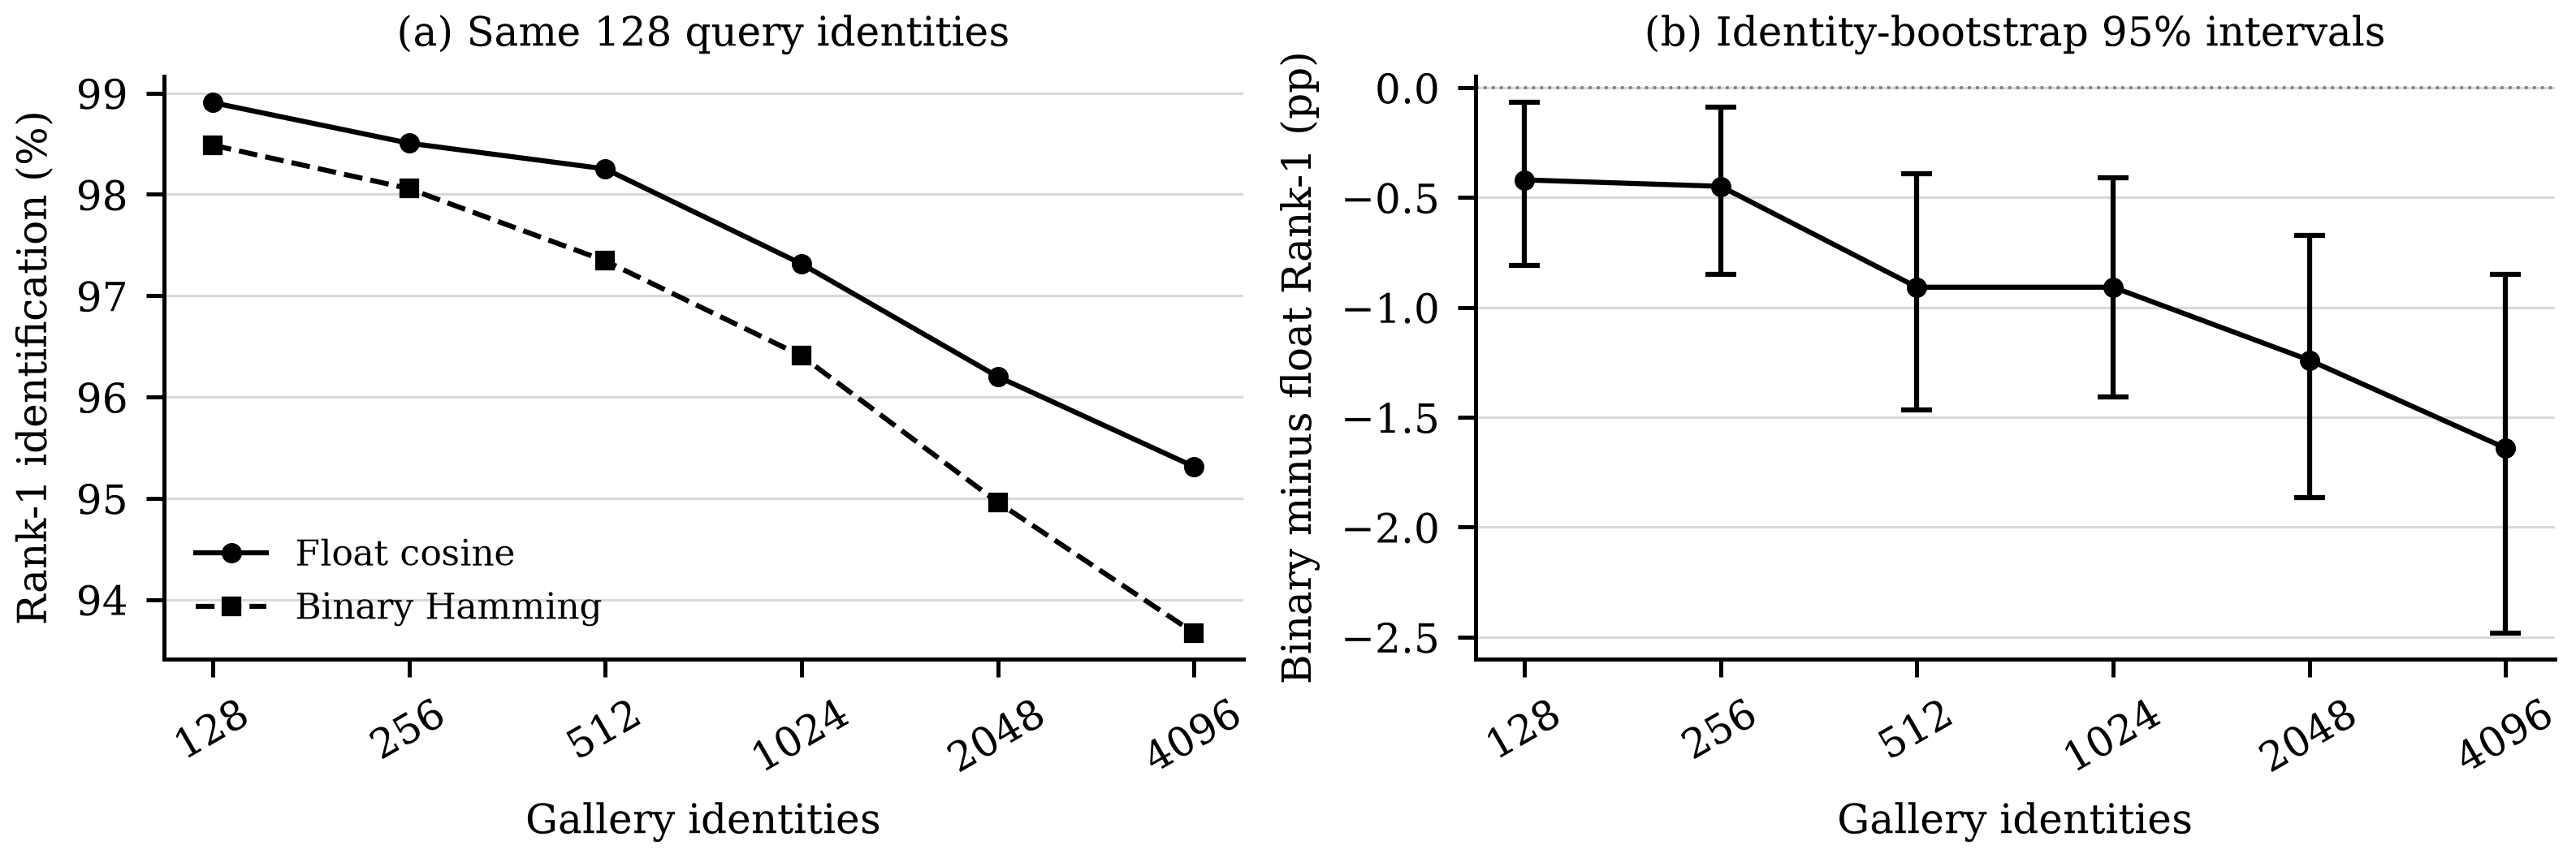
\includegraphics[width=\textwidth]{figures/lfw_paired_scale.png}\caption{Paired utility on nested LFW galleries, using the same 128 query identities and 20 gallery/probe assignments. Additional gallery identities are distractors. Intervals resample query identities after averaging repeated contexts; these are not 4096 independent query subjects.}\label{fig:paired_scale}\end{figure*}

At 128 identities, binarization costs 0.420 percentage points in Rank-1. At 4096, the loss is 1.641 points (binary-minus-float 95\% interval [-2.480, -0.850]). Masking adds no further score error, but it does not recover this frontend loss.

\subsection{Unenrolled Probes and Candidate Behavior}

\begin{table}[t]
\caption{Fresh-unknown LFW test: 512 calibration and 512 disjoint unknown identities. FPIR and DIR are percentages; rules are defined before feature extraction.}
\label{tab:open}\centering\small
\setlength{\tabcolsep}{3pt}
\begin{tabular}{rlrrr}
\toprule
Gallery & Root & Rule & FPIR & DIR \\
\midrule
128 & Float & Emp. & 1.602 & 89.26 \\
128 & Float & Cons. & 0.371 & 79.92 \\
128 & Binary & Emp. & 1.885 & 87.76 \\
128 & Binary & Cons. & 0.537 & 80.01 \\
4096 & Float & Emp. & 1.953 & 71.70 \\
4096 & Float & Cons. & 0.420 & 53.83 \\
4096 & Binary & Emp. & 1.172 & 59.12 \\
4096 & Binary & Cons. & 0.391 & 46.33 \\
\bottomrule
\end{tabular}
\end{table}

The nominal 1\% empirical calibration rule does not guarantee 1\% test FPIR. Conservative thresholds reduce false positives at a substantial DIR cost (Table~\ref{tab:open}). Identity-level intervals and all intermediate gallery sizes are retained in the supplement. The earlier 32-identity frequent-image pilot has test FPIR 5.34\% (float) and 7.19\% (binary) at its nominal 1\% target. This distinct hard population is not replaced or pooled with the confirmation cohort.

\begin{table}[t]
\caption{Unbounded candidate union on one frozen LFW split. Capacity-failing rows are diagnostics, not admitted secure indices.}
\label{tab:index}\centering\small
\setlength{\tabcolsep}{3pt}
\begin{tabular}{rrrrrr}
\toprule
Gallery & $w$ & Recall & Agreement & Fraction & Fallback \\
\midrule
128 & 4 & 1.0000 & 1.0000 & 0.9980 & 0.0566 \\
128 & 8 & 0.9941 & 0.9980 & 0.3049 & 0.9570 \\
4096 & 4 & 1.0000 & 1.0000 & 0.9980 & 0.1758 \\
4096 & 8 & 0.9941 & 0.9980 & 0.2893 & 0.9570 \\
\bottomrule
\end{tabular}
\end{table}

Four-bit buckets retrieve almost the complete gallery. At 4096 identities, eight-bit buckets retrieve about 29\%, but the exactness certificate invokes fallback on 95.70\% of probes. Their public capacity is 72 versus a required 138, with 59 overflowing buckets; enrollment must reject or reconfigure. The certified policy agrees with exhaustive decisions for every evaluated probe. The secure reference hides its choice by computing the full schedule, so candidate pruning is not a measured speedup.

\subsection{Relation Integrity and Leakage Diagnostics}

All eight injected faults are rejected, the previous logical state is retained, and the post-rejection query agrees with the independent oracle. Primitive tests also agree at full field width. In the retained SHAKE simulation, direct linkage AUC is 0.4948, direct assignment 0.0066 and relational assignment 0.0082, against chance 1/128 for assignment; the global-mask relational control is 1.0000. These are attack-specific observations, not an exposed-key or general irreversibility proof.

\subsection{Complete Secure Cost}

\begin{table}[t]
\caption{Input-inclusive five-party masked-system reference: mean and sample SD of three VM timings, global traffic (MB) and largest-child peak RSS (MiB). Five colocated processes; no WAN claim.}
\label{tab:secure}\centering\small
\setlength{\tabcolsep}{3pt}
\begin{tabular}{rlrrr}
\toprule
$N$ & Operation & Seconds & MB & RSS \\
\midrule
8 & Re-key & 9.82$\pm$1.30 & 471.8 & 38.7 \\
8 & Query & 2.28$\pm$0.05 & 10.9 & 27.6 \\
16 & Re-key & 10.05$\pm$0.35 & 722.6 & 48.3 \\
16 & Query & 1.71$\pm$0.25 & 18.3 & 32.9 \\
32 & Re-key & 12.41$\pm$1.51 & 997.3 & 60.0 \\
32 & Query & 2.08$\pm$0.40 & 33.2 & 38.0 \\
64 & Re-key & 16.77$\pm$0.19 & 1564.0 & 93.5 \\
64 & Query & 2.30$\pm$0.07 & 63.4 & 53.0 \\
128 & Re-key & 28.54$\pm$2.37 & 2717.4 & 132.8 \\
128 & Query & 4.09$\pm$0.35 & 122.5 & 63.1 \\
256 & Re-key & 44.02$\pm$0.31 & 5051.5 & 209.6 \\
256 & Query & 8.35$\pm$0.42 & 245.0 & 89.5 \\
\bottomrule
\end{tabular}
\end{table}

\begin{table}[t]
\caption{Complete lifecycle from each party's own persisted share file. Mean and sample SD of three measured VM timings; global MB. No plaintext database/index or old keys are resupplied to a computing party.}
\label{tab:persisted}\centering\small
\setlength{\tabcolsep}{3pt}
\begin{tabular}{rllrr}
\toprule
$N$ & State & Operation & Seconds & MB \\
\midrule
8 & Masked & Re-key & 10.73$\pm$2.15 & 470.7 \\
8 & Shared root & Re-key & 7.84$\pm$0.84 & 453.6 \\
8 & Masked & Query & 2.24$\pm$0.28 & 10.8 \\
8 & Shared root & Query & 0.40$\pm$0.07 & 0.9 \\
128 & Masked & Re-key & 40.76$\pm$6.51 & 2710.0 \\
128 & Shared root & Re-key & 30.36$\pm$4.51 & 2485.3 \\
128 & Masked & Query & 6.63$\pm$1.55 & 120.4 \\
128 & Shared root & Query & 1.22$\pm$0.21 & 14.6 \\
\bottomrule
\end{tabular}
\end{table}

The persisted-state implementation loads the complete public-size bundle before computing. Its helper functions and transition/query tail are source-identical to the input-inclusive reference; only the state entry point differs. Initialization uses an external trusted fixture that sends each party one degree-two Shamir evaluation per field. Repeated re-keying and reload queries agree with the oracle; exact/reject controls and rollback followed by reload also pass. The fixture is outside the computing-party corruption model.

At $N=128$, logical masked state is 3.506 MiB per party before serialization. Phase timers separate locator/index evolution, old/new masks, verification, selection, shuffle/refresh and fresh query masks; the supplement gives all components and wall times.

\begin{table}[t]
\caption{Input-inclusive same-configuration baselines and private indexed-query reference. Three measured runs after warmup; mean and sample SD. Full phase details accompany the logs.}
\label{tab:baselines}\centering\small
\setlength{\tabcolsep}{3pt}
\begin{tabular}{rllrr}
\toprule
$N$ & Design & Operation & Seconds & MB \\
\midrule
8 & Raw roots & Re-key & 5.74$\pm$0.27 & 454.8 \\
8 & Raw roots & Query & 0.50$\pm$0.16 & 1.0 \\
8 & Private index & Query & 43.28$\pm$0.86 & 4965.0 \\
32 & Raw roots & Re-key & 11.03$\pm$1.15 & 939.1 \\
32 & Raw roots & Query & 0.48$\pm$0.03 & 4.2 \\
128 & Raw roots & Re-key & 22.49$\pm$0.54 & 2492.7 \\
128 & Raw roots & Query & 0.91$\pm$0.05 & 16.7 \\
8 & Compact sort & Re-key & 93.88$\pm$22.51 & 7274.6 \\
16 & Compact sort & Re-key & 127.35$\pm$4.56 & 15788.2 \\
\bottomrule
\end{tabular}
\end{table}

An input-inclusive cost model fitted only at $N=8,16,32$ is checked on held-out measured sizes. Maximum relative error is 1.5\% for global communication and 86.9\% for local VM time. Exact residuals are reported even when the model is inaccurate; we make no extrapolated runtime claim at 4096. This model excludes persisted-file loading. The biometric 4096-gallery study is separate from measured MPC scale.


\section{Discussion and Limitations}
The experiments separate three questions: does masking preserve a given binary comparison; does the candidate index retrieve enough records; and how much biometric information is lost before protection? Algebra answers the first exactly. Candidate recall, certified fallback and float/binary comparisons answer the others empirically. A cheap-looking candidate union can contain almost the entire gallery, while more selective buckets can lose winners or overflow. The protected fixed-scan fallback restores exhaustive decisions but does not reduce query work.

Similarly, a correct transition does not imply a universally preferable representation. Shared roots plus refresh are simpler and already confidential under the same MPC threshold. Conventional encryption and updatable encryption offer established renewal options. The extra masked layer is useful when exposed logical template values must remain pseudorandom while their keys are hidden, and when the joint template/index transaction is the desired system boundary. The current measurements quantify that choice; they do not establish a general advantage over encrypted-search systems.

The prototype uses passive MPC, one encoder and custom public-dataset protocols, with five colocated processes. The MiMC security assumption is explicit, not independently proven here. The access-hiding backend uses fixed scans and secret row shuffles, not an efficient ORAM. Logical atomicity does not cover distributed crash recovery. Strong post-compromise encryption security, active-party attacks, demographic performance, modern generative reconstruction and large-scale operational deployment require further work. The 512 unknown test identities do not support claims at FPIR $10^{-3}$ or lower.

\section{Ethical Considerations}
Only public research datasets are used under their providers' access conditions. Local caches and derived biometric features remain sensitive and are not automatically redistributed. Template protection does not remove surveillance or exclusion risks; any operational use requires purpose limitation, retention controls and human review for consequential decisions.

\section{Conclusion}
\MSLE specifies and implements a joint renewal invariant for masked binary templates and a private index. Its exactness is conditional on the compared candidate set; its confidentiality requires secret keys and protected metadata. The revised evaluation measures binarization loss, candidate behavior and complete secure-system cost, and positions the design against simpler shared roots and an oblivious transition baseline. These boundaries make the lifecycle contribution testable without conflating score preservation, retrieval completeness or encrypted-search efficiency.

\section*{Acknowledgment}
This research has been funded by the Committee of Science of the Ministry of Science and Higher Education of the Republic of Kazakhstan (Grant No. BR24992852, ``Intelligent models and methods of Smart City digital ecosystem for sustainable development and the citizens' quality of life improvement'').
\section*{Data and Code Availability}
The original released artifact is at \url{https://github.com/theossenovserzhan/sle-reproducibility}. The accompanying revision archive contains corrected sources, frozen parameters, protocol manifests, image/feature checksums, raw logs and scripts producing every new table. Face images and locally extracted embeddings are excluded; reproduction obtains source data from their providers.
\bibliographystyle{IEEEtran}\bibliography{references}
% Author biographies and photos retained from the supplied author materials.

\begin{IEEEbiography}[{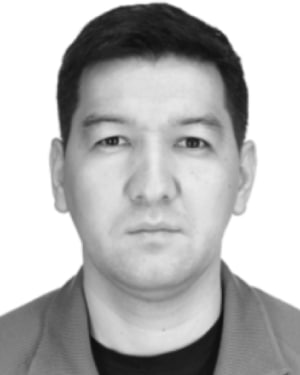
\includegraphics[width=1in,height=1.25in,clip,keepaspectratio]{author_photo_beibut_amirgaliyev.png}}]{Beibut Amirgaliyev}
(Member, IEEE) received the B.S. degree in information systems from Kazakh-British Technical University, and the M.S. degree in software engineering and the Ph.D. degree in computer science and mathematical modeling from the Kazakh National Technical University, Almaty, Kazakhstan. From 2010 to 2018, he was an Assistant Professor with International Information Technology University. Since 2019, he has been a Professor with the Department of Computer Engineering, Astana IT University. He has authored more than 40 papers indexed in Scopus and Web of Science. His research interests include smart city applications, machine learning, and innovation. He is Executive Editor of the Scientific Journal of Astana IT University.
\end{IEEEbiography}

\begin{IEEEbiography}[{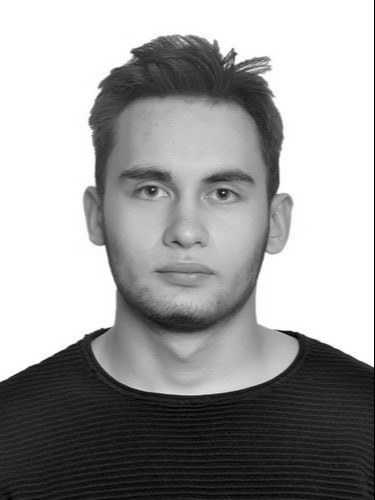
\includegraphics[width=1in,height=1.25in,clip,keepaspectratio]{author_photo_serzhan_ossenov.jpg}}]{Serzhan Ossenov}
(Member, IEEE) received the B.S. degree in Big Data Analysis from Astana IT University, Astana, Kazakhstan, in 2025. He is currently pursuing the M.S. degree in Applied Data Analytics at Astana IT University. Since 2026, he has been a Big Data Analyst with the National Bank of Kazakhstan, specializing in data quality and data governance. His research interests include privacy-preserving machine learning, image recognition, federated learning, differential privacy, and data quality.
\end{IEEEbiography}

\end{document}
